\chapter{Modelos Lineales}

\section{Algoritmo de aprendizaje del Perceptrón (PLA)}

Implementar la función 
\mintinline{python}{ajusta_PLA(datos, label, max_iter, vini)} 
que calcula el  hiperplano solución a un problema de clasificación binaria
usando el algoritmo PLA. La entrada datos es una matriz donde cada item con su
etiqueta está representado por una fila de la matriz, label el vector de
etiquetas (cada etiqueta es un valor $+1$ o $-1$), \mintinline{python}{max_iter}
es el número máximo de iteraciones permitidas y vini el valor inicial del vector.
La función devuelve los coeficientes del hiperplano.

\subsection{Ejecutar el algoritmo PLA con los datos empleados en el apartado 2a del
ejercicio 1.}

Inicializar el algoritmo con: 

\begin{itemize}
\item el vector cero y, 
\item con vectores de números aleatorios en [0, 1] (10 veces).
\end{itemize}

Anotar el número medio de iteraciones necesarias en ambos para converger.

Se deben mostrar en una tabla cada uno de los pesos iniciales empleados, los
finales (obtenidos tras el proceso de entrenamiento), y el porcentaje de error
de clasificación. \textbf{Valorar el resultado relacionando el punto de inicio con el
número de iteraciones.}

\hfill \break

El algoritmo de aprendizaje del perceptrón (PLA) implementado en
\mintinline{python}{ajusta_PLA} consiste en actualizar los pesos por cada punto
mal clasificado de la muestra de acuerdo a la siguiente regla:

$$
w(t+1) = w(t) + x_i \cdot y_i
$$

Esto se hace hasta que el vector de pesos no cambie en toda una época (recorrido
de la muestra) o se alcance el número máximo de iteraciones \mintinline{python}{max_iter}.
La implementación realizada devuelve el histórico de pesos, el número de
iteraciones dadas y el error de clasificación.

Para visualizar el proceso de convergencia de PLA, se ha implementado una clase 
\mintinline{python}{Animacion}. En la ejecución del código se muestra esta
animación para el vector inicial nulo en los datos sin ruido, donde tras $75$
iteraciones se encuentra un clasificador con $0\%$ de error.

\begin{table}[!ht]
    \centering
    \begin{tabular}{llll}
    \toprule
        Vector inicial & Iteraciones & Coeficientes w & Error de clasificación \\ \midrule
        $[0.000, 0.000, 0.000]$ & $75$ & $[661.00,23.20,32.39]$ & $0\%$ \\ \midrule
        $[0.574, 0.349, 0.057]$ & $257$ & $[1115.57,43.48,62.12]$ & $0\%$ \\
        $[0.229, 0.664, 0.497]$ & $43$ & $[464.23,15.39,23.75]$ & $0\%$ \\ 
        $[0.519, 0.175, 0.571]$ & $231$ & $[1078.52,39.47,53.76]$ & $0\%$ \\
        $[0.997, 0.817, 0.594]$ & $71$ & $[664.00,23.15,31.90]$ & $0\%$ \\ 
        $[0.976, 0.902, 0.596]$ & $76$ & $[661.98,24.90,36.20]$ & $0\%$ \\ 
        $[0.032, 0.094, 0.065]$ & $59$ & $[558.03,19.36,29.71]$ & $0\%$ \\ 
        $[0.452, 0.375, 0.975]$ & $274$ & $[1145.45,40.28,60.81]$ & $0\%$ \\
        $[0.168, 0.973, 0.767]$ & $235$ & $[1089.17,39.45,53.53]$ & $0\%$ \\
        $[0.824, 0.633, 0.669]$ & $257$ & $[1148.82,39.90,60.95]$ & $0\%$ \\
        $[0.477, 0.013, 0.353]$ & $74$ & $[673.48,22.59,31.35]$ & $0\%$ \\ \bottomrule
        Promedio & $157.7$ & ~ & $0\%$ \\ \bottomrule
    \end{tabular}
    \caption{Resultados de ejecución de PLA \textbf{muestra sin ruido} para vector inicial nulo y generados aleatoriamente (10 iteraciones)}
\end{table}

Podemos observar en los resultados, que al ser los datos \textbf{linealmente separables}, 
PLA converge en todos los casos a una recta con error de clasificación cero en
una media de $\approx 158$ iteraciones (vectores iniciales aleatorios).

Si hallamos la desviación típica del número de iteraciones, obtenemos $94.17$, un valor
considerablemente alto que indica la alta sensibilidad de la convergencia (nº de iteraciones
en llegar al $0\%$ de error) con respecto al vector inicial. Podemos afirmar por
tanto, que escoger el vector nulo como vector inicial resulta ser una buena heurística.

En las siguiente figura, vemos los clasificadores obtenidos para el vector nulo, el vector
generado aleatoriamente en la iteracion $7$ y el clasificador original. Le sigue una gráfica
para visualizar la disminución del error de clasificación a lo largo de las iteraciones.

\begin{figure}[H]
  \caption{Muestra linealmente separable (sin ruido)}\par\medskip
  \begin{minipage}[b]{.5\linewidth}
    \centering
    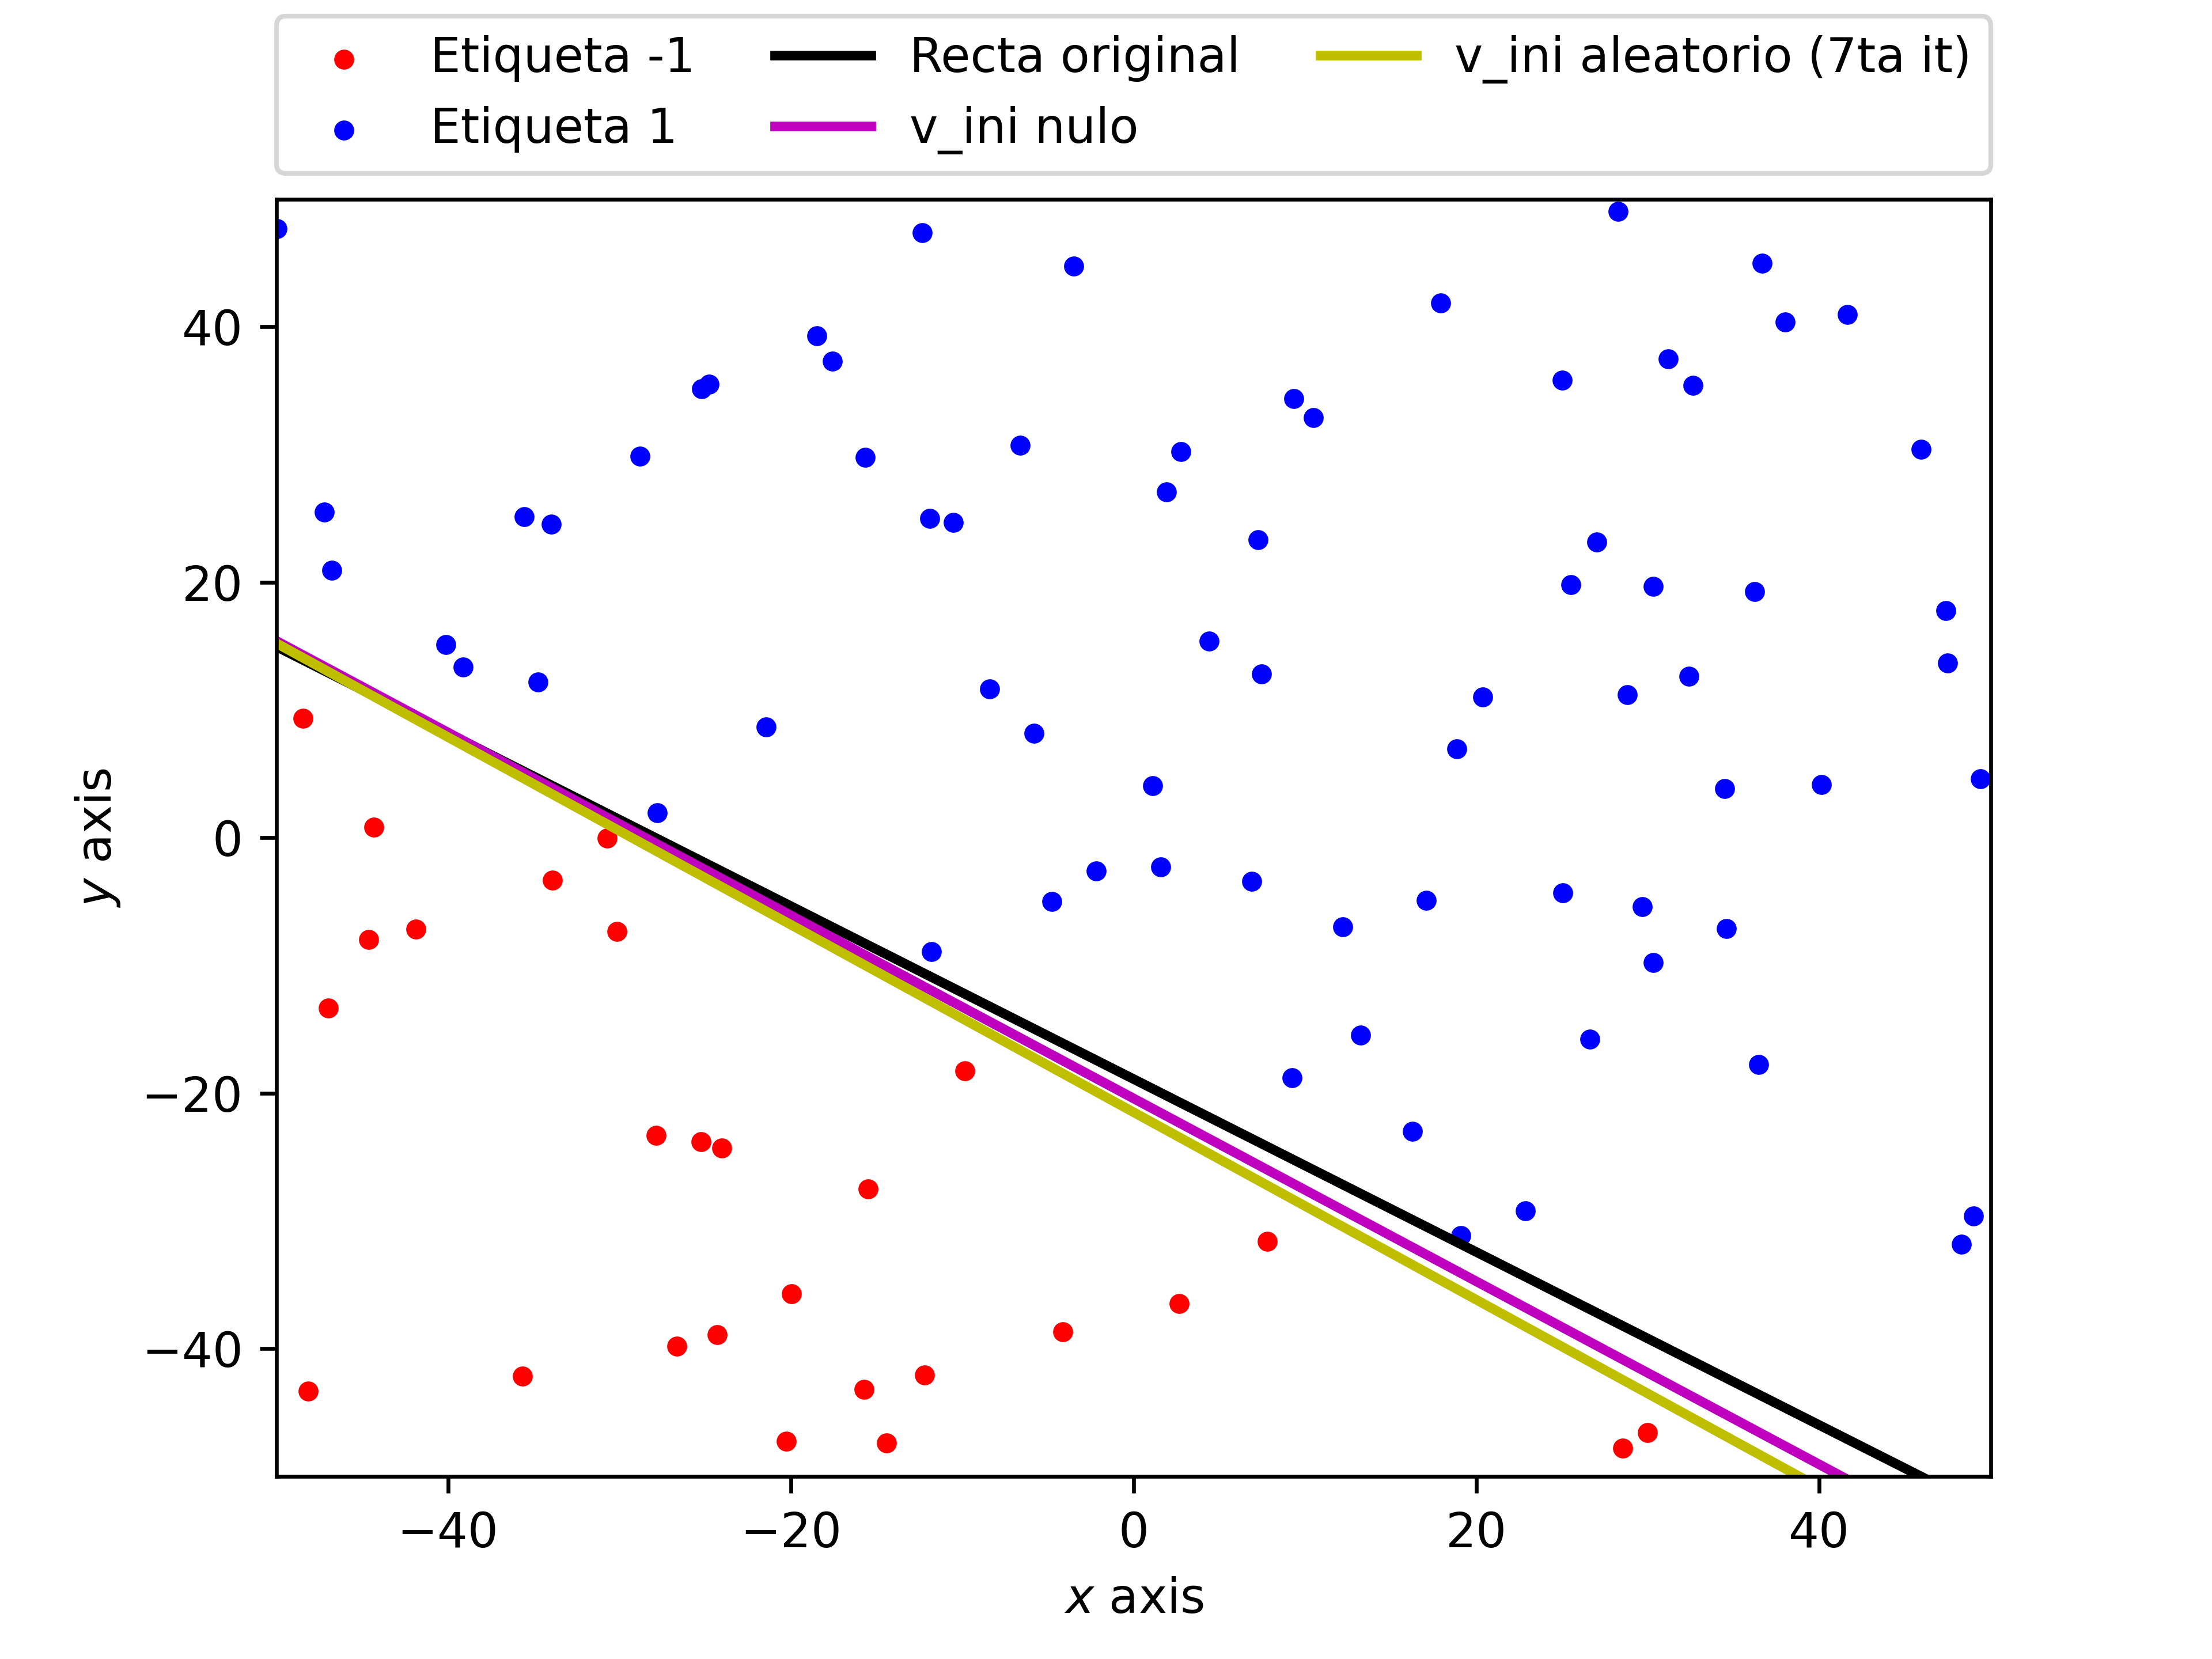
\includegraphics[width=0.9\textwidth]{Figure_10}
    \subcaption{Clasificadores para distintos \mintinline{python}{v_ini}} \label{subfig-4:dummy2}
  \end{minipage}
  \hfill \hfill
  \begin{minipage}[b]{.5\linewidth}
    \centering
    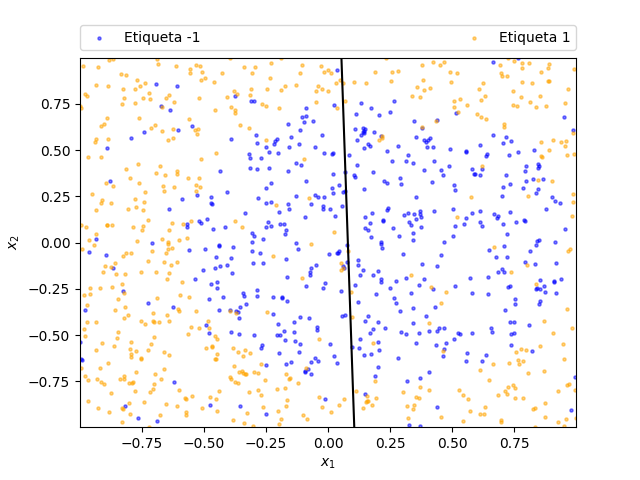
\includegraphics[width=0.95\textwidth]{Figure_9}
    \subcaption{\% Error clasif. a lo largo de las épocas}
  \end{minipage}
  \label{fig:dummy3}
\end{figure}

\subsection{Repetir usando los datos del apartado 2b del ejercicio 1.}
\textbf{¿Observa algún comportamiento diferente? En caso afirmativo diga cuál y las
razones para que ello ocurra.}

\begin{figure}[H]
  \caption{Muestra con ruido (no linealmente separable)}\par\medskip
  \begin{minipage}[b]{.5\linewidth}
    \centering
    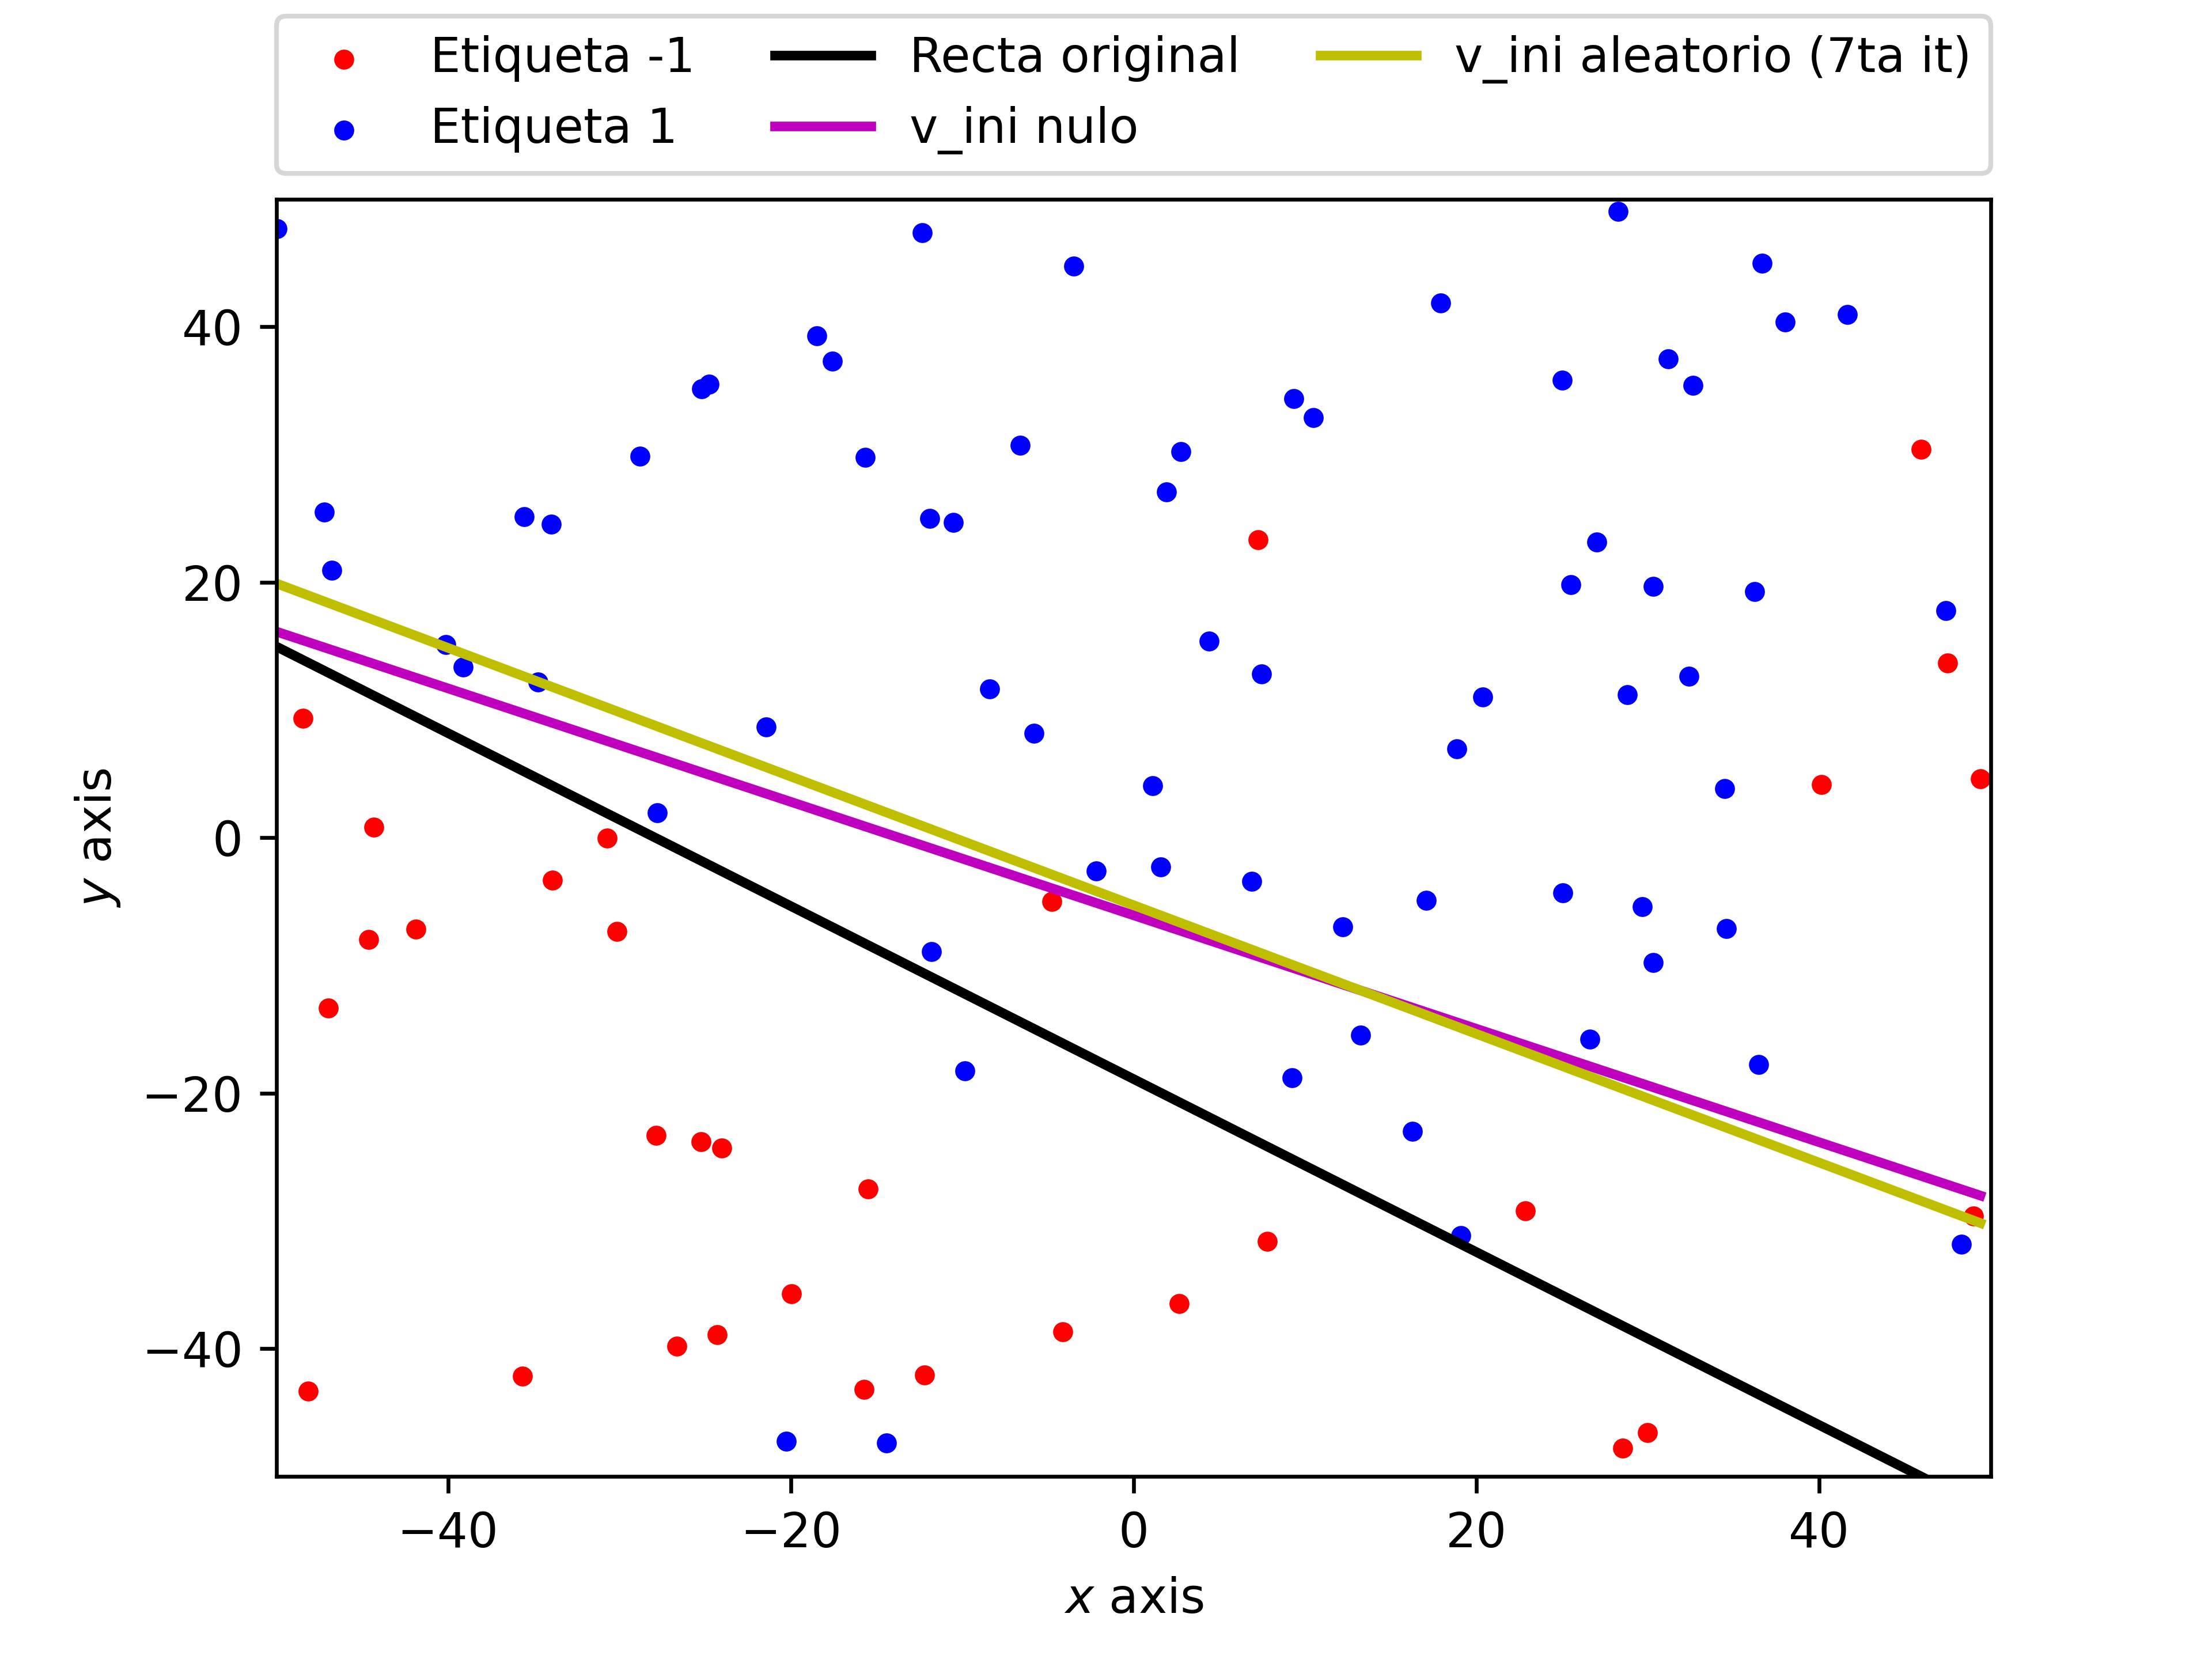
\includegraphics[width=0.9\textwidth]{Figure_12}
    \subcaption{Clasificadores para distintos \mintinline{python}{v_ini}} \label{subfig-4:dummy6}
  \end{minipage}
  \hfill \hfill
  \begin{minipage}[b]{.5\linewidth}
    \centering
    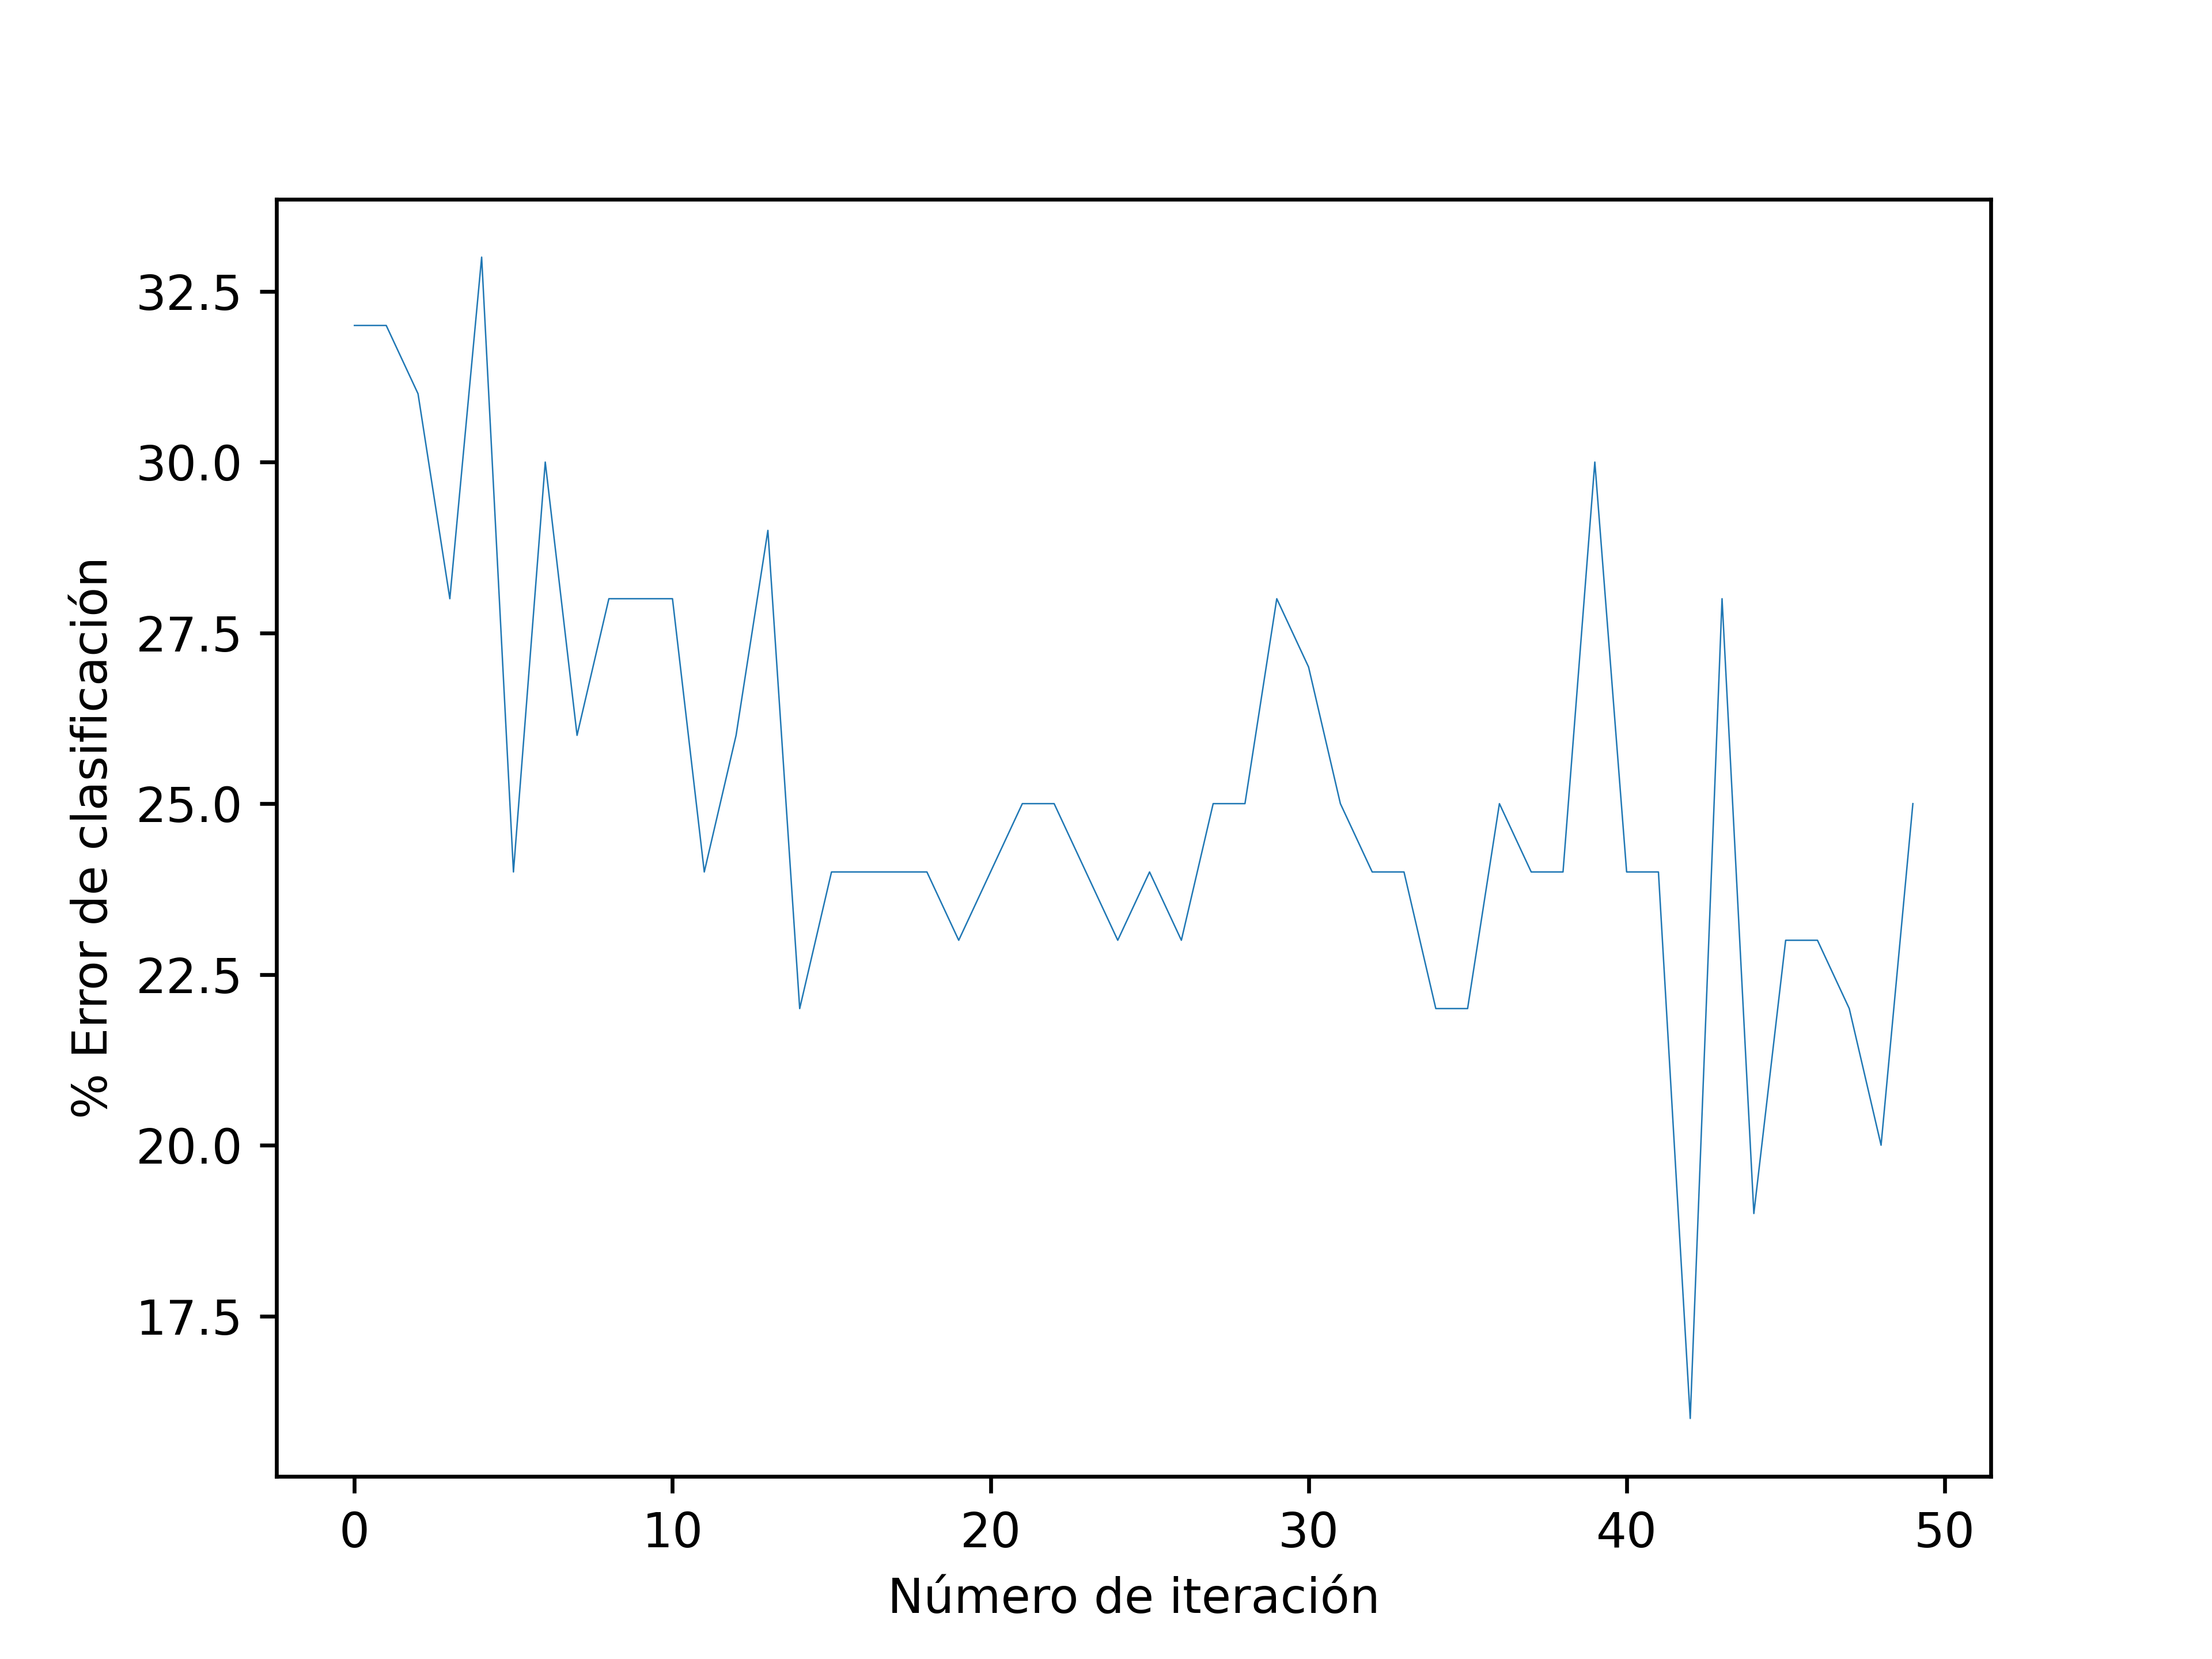
\includegraphics[width=0.95\textwidth]{Figure_11}
    \subcaption{\% Error clasif. a lo largo de las épocas}
  \end{minipage}
  \label{fig:dummy9}
\end{figure}


En este caso, partimos de la muestra de datos con $10\%$ de ruido. Así, PLA no tiene
garantizada una convergencia pues los datos \textbf{no son linealmente separables} y 
la cota inferior del error de clasificación para las rectas obtenidas con PLA
es justo ese $10\%$.

Por tanto, las ejecución se para al alcanzar el máximo número de iteraciones (épocas)
que se ha fijado en $5000$.


\begin{table}[H]
    \centering
    \begin{tabular}{llll}
    \toprule
        Vector inicial & Iteraciones & Coeficientes w & Error de clasificación \\ \midrule
        $[0.000, 0.000, 0.000]$ & $5000$ & $[339.00,24.81,55.86]$ & $24\%$ \\ \midrule
        $[0.492, 0.730, 0.469]$ & $5000$ & $[348.49,17.77,42.43]$ & $24\%$ \\ 
        $[0.457, 0.138, 0.011]$ & $5000$ & $[349.46,16.66,44.13]$ & $24\%$ \\ 
        $[0.758, 0.320, 0.984]$ & $5000$ & $[339.76,21.61,56.29]$ & $22\%$ \\ 
        $[0.220, 0.339, 0.524]$ & $5000$ & $[336.22,17.72,43.85]$ & $25\%$ \\ 
        $[0.755, 0.464, 0.125]$ & $5000$ & $[336.75,17.32,53.11]$ & $27\%$ \\ 
        $[0.313, 0.505, 0.674]$ & $5000$ & $[339.31,15.10,26.87]$ & $20\%$ \\ 
        $[0.770, 0.130, 0.023]$ & $5000$ & $[333.77,27.72,49.69]$ & $20\%$ \\ 
        $[0.519, 0.810, 0.013]$ & $5000$ & $[343.52,12.09,38.81]$ & $22\%$ \\ 
        $[0.672, 0.687, 0.449]$ & $5000$ & $[331.67,12.87,21.73]$ & $19\%$ \\ 
        $[0.915, 0.644, 0.005]$ & $5000$ & $[341.91,21.10,56.13]$ & $22\%$ \\ \bottomrule
        Promedio & $5000$ & ~ & $22.5\%$ \\ \bottomrule
    \end{tabular}
    \caption{Resultados de ejecución de PLA \textbf{muestra con ruido} para vector inicial nulo y generados aleatoriamente (10 iteraciones)}
\end{table}

Al contrario que en el caso anterior (muestra sin ruido), ejecutar el algoritmo 
con vector nulo como vector inicial produce un error de clasificación mayor que
la media obtenida para los 10 vectores iniciales generados aleatoriamente 
($24\%$ vs $22.5\%$). Además, en este caso, por lo comentado anteriormente,
el vector inicial no influye en el número de iteraciones.

En cuanto a la variación del error por número de iteraciones, podemos observar grandes
oscilaciones, estando concentrados la mayoría en el intervalo $22.5 \pm 2.5\%$. 
El mínimo se alcanza entorno a la iteración $4000$ donde el error llega a ser
$14\%$, bastante cerca de la cota inferior del $10\%$ antes mencionada.

\section{Regresión Logística (RL)}

En este ejercicio emplearemos nuestra propia función objetivo $f$ y un conjunto
de datos $D$ para ver cómo funciona regresión logística. Consideraremos d = 2
para que los datos sean fácilmente visualizables, y emplearemos 
$X = [0, 2] \times [0, 2]$ con probabilidad uniforme de elegir cada $x \in X$.
Elegir una línea en el plano que pase por X como la frontera que separa la
región en donde y toma valores $+1$ y $-1$.

Para ello, seleccionar dos puntos aleatorios de $X$ y calcular la línea que pasa
por ambos.

Impleméntese RL con Gradiente Descendente Estocástico (SGD) del siguiente modo:

\begin{itemize}
\item Inicializar el vector de pesos con valores 0.
\item Parar el algoritmo cuando $\Vert w(t+1) - w(t) \Vert < 0.01$, donde $w(t)$
denota el vector de pesos al final de la época $t$. Recuérdese que una época es
un pase completo a través de los N ejemplos de nuestro conjunto de datos. 
\item Aplicar una permutación aleatoria de $\{1, 2,..., N\}$ a los índices de
los datos, antes de usarlos en cada época del algoritmo. 
\end{itemize}

A continuación, empleando la implementación anterior, realícese el siguiente
experimento: 

\begin{itemize}
\item Seleccione $N = 100$ puntos aleatorios $\{x_n \}$  de $X$ y evalúe las
respuestas $\{y_n \}$ de todos ellos respecto de la frontera elegida.
\item Ejecute RL para encontrar la función solución $g$, y evalúe el error 
$E_{out}$ usando para ello una nueva muestra de datos ($> 999$). Se debe
escoger experimentalmente tanto el learning rate (tasa de aprendizaje $\eta$)
como el tamaño de batch. 
\item Repita el experimento $100$ veces, y calcule los valores promedio de 
$E_{out}$, de porcentaje de error de clasificación, y de épocas necesarias para
converger.
\end{itemize}

\hfill \break

Recordamos que la Regresión Logística es un modelo lineal de clasificación,
donde ahora la función hipótesis es de la forma

\begin{equation}
h(x) = \theta(w^T X)
\end{equation}

con $\theta(s) = \frac{e^s}{1 + e^s} = \frac{1}{1 + e^{-s}}$ la llamada
\textbf{función logística o sigmoide} que toma valores en $[0, 1]$. Estos se
interpretan de forma probabilística para un evento binario.
A través del método de máxima verosimilitud (\cite{LFD}), obtenemos 
una medida de error en la muestra:

\begin{equation}
E_{in}(w) = \frac{1}{N} \sum_{n=1}^N \ln(1 + e^{y_n w^T x_n})
\end{equation}

Intuitivamente, el error se acerca más a cero cuanto mayor es cada
$y_n w^T x_n$ (positivo). Esto implicaría que $\text{sign}(w^T x_n) = y_n$,
es decir, un número mayor de instancias $x_n$ bien clasificadas.

Para entrenar el modelo, aplicamos \textbf{gradiente descendente estocástico (SGD)}
en su versión \textbf{batch de 1 elemento}. Es decir, por cada época hallamos una
permutación de las instancias $x_n$ (índices en la implementación), computamos
el gradiente de cada instancia y actualizamos los pesos. La expresión del gradiente
para batch de tamaño $M=1$ es (\cite{LFD}):

\begin{equation}
  \nabla E_{in}(w) = \frac{-1}{M} \sum_{n=1}^M \frac{y_nx_n}{1+e^{y_n w^T x_n}} = \frac{-y_n x_n}{1+e^{y_n w^T x_n}}
\end{equation}

La implementación del algoritmo se encuentra en la función \\
\mintinline{python}{sgdRL(X, y, lr, max_iter, epsilon=0.01)} y se ha seguido el
criterio de parada descrito en el enunciado $\Vert w(t+1) - w(t) \Vert < 0.01$
parametrizando $0.01$ como \mintinline{python}{epsilon} por si se quisiera
experimentar con otros valores en un futuro.

En cuanto a la realización del experimento, se ha decidido generar la muestra de test
$X_{test}$ con $1000$ elementos ($> 999$) para no incrementar demasiado el tiempo
de ejecución en las $100$ repeticiones. Todas las llamadas al algoritmo de aprendizaje
de Regresión Lineal se han realizado con un \textbf{learning rate $\eta = 0.01$, un número máximo
de $1000$ iteraciones y tamaño de batch de $1$ elemento.}

En efecto, se ha comprobado experimentalmente que valores mayores de $\eta$
$(0.2, 0.4, 0.6)$ implican un mayor número de iteraciones debido al criterio de
parada (la distancia entre los vectores de pesos tarda más en disminuir), aunque
menor error $E_{in}$.

Por otro lado, se implementó inicialmente el algoritmo de aprendizaje de
regesión logística en su versión SGD minibatch con tamaño de batch superiores a $1$
$(2, 4, 16, 32, 64)$, ofreciendo menor número de épocas aunque mayor error.

\begin{table}[H]
    \centering
    \begin{tabular}{llll}
    \toprule
        Repetición & $E_{out}$ & $E_{out}^{clas}$ (\%) & Épocas para converger \\ \midrule
        $0$ & $0.099$ & $0.8 \%$ & $373$ \hfill \\
        $1$ & $0.094$ & $0.7 \%$ & $411$ \hfill\\
        $2$ & $0.136$ & $0.9 \%$ & $536$ \hfill \\
        $3$ & $0.107$ & $0.2 \%$ & $415$ \hfill \\
        $4$ & $0.099$ & $2.7 \%$ & $399$ \hfill \\
        $5$ & $0.118$ & $0.7 \%$ & $473$ \hfill \\
        $\dots$ & $\dots$ & $\dots$ & $\dots$ \hfill \\
        $95$ & $0.122$ & $4.0 \%$ & $283$ \hfill \\
        $96$ & $0.095$ & $1.7 \%$ & $374$ \hfill \\
        $97$ & $0.108$ & $0.8 \%$ & $426$ \hfill \\
        $98$ & $0.145$ & $2.3 \%$ & $476$ \hfill \\
        $99$ & $0.146$ & $4.7 \%$ & $410$ \hfill \\ \bottomrule
        \textbf{Promedio} & \textbf{$0.117$} & \textbf{$2.46 \%$} & \textbf{$413.25$} \\ \bottomrule
    \end{tabular}
    \caption{Resultados de ejecución de 100 experimentos de Regresión Logística}
\end{table}